\documentclass[12pt, a4paper, oneside]{ctexbook}
\CTEXsetup[format={\Large\bfseries}]{section}
\usepackage{amsmath, amsthm, amssymb, bm, graphicx, hyperref, mathrsfs}
\usepackage{float}
\usepackage{graphicx}
\usepackage{geometry}
\usepackage{enumerate}
\usepackage{multirow}
\usepackage{subfigure}
\usepackage{caption}
\usepackage{color}
\usepackage{cite}
\usepackage{setspace}
\usepackage{appendix}
\usepackage{listings}
\usepackage{xcolor}
\lstset{ 
  backgroundcolor=\color{white},   % 选择代码背景,必须加上\ usepackage {color}或\ usepackage {xcolor}.
  basicstyle=\footnotesize,        % 设置代码字号.
  breakatwhitespace=false,         % 设置是否当且仅当在空白处自动中断.
  breaklines=true,                 % 设置自动断行.
  captionpos=b,                    % 设置标题位置.
  commentstyle=\color{green},      % 设置注释格式
  deletekeywords={...},            % 是否删除给定语言的关键词.
  extendedchars=true,              % 是否允许使用非ASCII字符; 仅适用于8位编码,不适用于UTF-8. 
  frame=single,	                   % 给代码区添加边框.
  keepspaces=true,                 % 保留空格(useful for keeping indentation of code (possibly needs columns=flexible).
  keywordstyle=\color{blue},       % 关键字显示风格.
  language=matlab,                 % 使用的语言.
  morekeywords={*,...},            % 是否需要添加其他的关键词.
  numbers=left,                    % 给代码添加行号,可取值none, left, right.
  numbersep=5pt,                   % 设置行号与代码之间的间隔
  numberstyle=\tiny\color{gray}, % 行号的字号和颜色
  rulecolor=\color{black},         % 边框颜色,如果没有设置,框架颜色可以在非黑色文本中的换行符上更改(例如 text (e.g. comments (green here)))
  showspaces=false,                % 显示每个地方添加特定下划线的空格; 覆盖了'showtringspaces'
  showstringspaces=false,          % 仅在字符串中允许空格
  showtabs=false,                  % show tabs within strings adding particular underscores
  stepnumber=1,                    % the step between two line-numbers. If it's 1, each line will be numbered
  stringstyle=\color{mymauve},     % string literal style
  tabsize=2,	                   % 将默认tab设置为2个空格
  title=\lstname                   % show the filename of files included with \lstinputlisting; also try caption instead of title
}
\geometry{a4paper,scale=0.8}
\setcounter{secnumdepth}{4}  %%  设置标题级别深度
\setcounter{tocdepth}{3}  %%  设置目录深度
%%  文索引文献上标
\makeatletter
\def\@cite#1#2{\textsuperscript{[{#1\if@tempswa , #2\fi}]}}
\makeatother
%\renewcommand\thetable{\alph{table}}
%%  上述部分式导入一部分宏包,请勿乱动;如有需要可自行添加宏包\usepackage


\hypersetup{hidelinks} %%  目录跳转超链接红框隐藏
\linespread{1.5} %%  全文行间距


%%  开始全文
\begin{document}

%% 导入封面:content文件夹下的cover.tex文件
%% 设计封面

\begin{titlepage}
    \centering

    %------------------------------------------------------------
    %    Top rules
    %------------------------------------------------------------

    \rule{\textwidth}{1pt}   % The top horizontal rule
    \vspace{0.01\textheight}  % Whitespace between top horizontal rule and title


    %------------------------------------------------------------
    %    Title
    %------------------------------------------------------------

    \begin{figure}[H]
    \centering
    
\includegraphics[width=0.15\textwidth]{logo/nuaa-logo-black.pdf}
    \end{figure}
    
    \begin{figure}[H]
    \centering
    
\includegraphics[width=0.6\textwidth]{logo/nuaa-jianqi.pdf}
    \end{figure}
    
    \vspace{0.02\textheight}
    
    {\Huge \textbf{飞机部件课程设计报告书}}
    

    \vspace{0.005\textheight}   % Whitespace between the title and short horizontal rule

    \rule{0.83\textwidth}{0.4pt}  % The short horizontal rule under title

    \vspace{0.05\textheight}  % Whitespace between the short horizontal rule and author

    %------------------------------------------------------------
    %    Author
    %------------------------------------------------------------

    {\Huge \textbf{题目:}XX方向舵设计}

    \vspace{0.03\textheight} 
    
    
    {\Huge \textbf{学生姓名:}包晨宇}
    
    \vspace{0.03\textheight} 

    {\Huge \textbf{学号:}011810422}

    \vspace{0.03\textheight} 
    
    {\Huge \textbf{学院:}航空学院}
    \vspace{0.03\textheight} 
    
    {\Huge \textbf{专业:}飞行器设计与工程}
    \vspace{0.03\textheight} 
    
    {\Huge \textbf{班级:}0118104}
    \vspace{0.03\textheight} 
    
    {\Huge \textbf{指导老师:}徐惠民}

    \vfill  % Whitespace between author and date

    {\Large \today}
    \vspace{0.02\textheight}  % Whitespace between date and bottom horizontal rule

    %------------------------------------------------------------
    %    Bottom rules
    %------------------------------------------------------------

    \rule{\textwidth}{1pt}  % The bottom horizontal rule

\end{titlepage}


%% 任务书封面

\newpage
\begin{centering}

    {\large 飞机部件课程设计任务书}

\end{centering}


\centerline{    
    班级:\underline{\quad\quad 0118104 \quad\quad}
    \quad\quad
    学号:\underline{\quad\quad 011810422 \quad\quad}
    \quad\quad
    姓名:\underline{\quad\quad 包晨宇 \quad\quad}
}

\noindent \textbf{题目名称:} XX方向舵设计



\begin{spacing}{1.0}
\noindent\textbf{内容和要求:}

\begin{enumerate}
    \item 完成设计计算工作,提供技术总结报告一份;
    \item 完成理论图、装配图、零件图、组件图的设计和绘制;
    \item 进行重量计算和配重设计,要求结构重心落在转轴上或前面1\%弦长位置内;
    \item 制订装配方案;
    \item 所设计的文件和图纸应符合国家或部标准、符合生产使用单位要求。
\end{enumerate}

\noindent\textbf{原始数据:}

\begin{itemize}
    \item 几何数据(见飞机部件课程设计计划书图三)
    \begin{enumerate}
        \item 平面几何尺寸及协调关系如图三;
        \item 方向舵XOY平面的外形由垂直尾翼翼型的后段和方向舵前段外形确定,见飞机部件课程设计计划书表1和表2;
        \item 方向舵最大偏度$\pm 15^{\circ}$;
        \item 方向舵几何外形见飞机部件课程设计计划书图三;
    \end{enumerate}

    \item 外载荷
    \begin{enumerate}
        \item 方向舵使用载荷:见飞机部件课程设计计划书;
        \item 展向分布规律按飞机部件课程设计计划书图1;
        \item 弦向分布规律按飞机部件课程设计计划书图2。
    \end{enumerate}
\end{itemize}

\noindent\textbf{参考资料:}

\begin{enumerate}
    \item 《飞机设计手册》第三册
    \item 《航空机械设计手册》
    \item 《航空材料标准手册》
    \item 《飞机零构件设计》
    \item 《飞机构造设计常用参考资料》
    \item 《军用飞机强度规范》
    \item 《机械制图》
    \item 《理论力学》
    \item 《材料力学》
\end{enumerate}
\end{spacing}

\vspace{0.02\textheight}
\centerline{    
    起止日期:\underline{2021.xx.xx$\sim$2021.xx.xx}
    \quad\quad
    指导老师:\underline{\quad\quad 徐惠民、王强 \quad\quad}
    \quad\quad
    成绩:\underline{\quad\quad\quad\quad\quad\quad\quad\quad}
}

%% 设置目录:自动生成
\newpage
\pagenumbering{Roman}
\setcounter{page}{1}
\tableofcontents  %%  目录设置
\newpage
\setcounter{page}{1}
\pagenumbering{arabic}

%%  开始正篇

%% 将content中的各个分开写好的章节全部用include命令加到正文重


%%  请打开content/帮你上手可删,我写了一些latex基本操作

\chapter{帮你上手可删}

听说你对latex使用不熟,下面给你书写一些基本操作

\section{这是章节内一级标题}

\subsection{这是章节内二级标题}

\subsubsection{这是章节内三级标题}


\section{列表}

\subsection{有序列表}

使用enumerate 命令

\begin{enumerate}
    \item 第一点
    \item 第二点
    \item 第三点
\end{enumerate}

\subsection{无序列表}

使用itemize 命令

\begin{itemize}
    \item 巴拉巴拉
    \item 淅沥淅沥
    \item 哗啦哗啦
\end{itemize}


\section{公式}

\subsection{行内公式}

使用美元符号\$将公式圈起来:$\frac{1}{2}mV^2=E_k$;

一段输入转矩$T_{1.in}$,最大功率$P_{\max}$等等

\subsection{行间公式}

如果需要编号,使用begin\{equation\}命令

\begin{equation}
    \alpha=\alpha_0+\frac{L_d-L}{2}
\end{equation}

latex自动为您编号:

\begin{equation}
    d_1\geq 76.6\left( \frac{K\cdot T_1}{\Psi_d^2[\sigma]_{H2}^2}\cdot\frac{\mu+1}{\mu} \right)^{\frac{1}{3}}
\end{equation}

若无需编号,使用双美元\$\$包围:

$$
v=\frac{\pi d n}{60\times 1000}
$$

\subsection{常用符号}

\begin{itemize}
    \item $\cos,\sin,\tan,\ln$:\textbackslash cos,\textbackslash sin,\textbackslash tan,\textbackslash ln(前加反斜杠)
    \item $\cdot$:cdot命令
    \item $\times$:times命令
    \item $x_a^b$:下标\_\{内容\},上标 \^{}\{内容\}
    \item $^{\circ}$:\^{} \{\textbackslash circ\}
    \item $\sqrt{x}$:\textbackslash sqrt命令
    \item $\frac{a}{b}$:分数,\textbackslash frac命令
    \item $P_{\text{许用}}$:汉字,使用\textbackslash text\{\}命令包裹汉字
    \item $\left( \frac{1}{3}\right)$:括号变大符号,使用left,right控制
    \item $\alpha,\beta,\Psi$:希腊字母,请用的时候查阅
    \item $\%$:latex里百分号意味着注释,使用前加上\textbackslash 反斜杠用以转义
\end{itemize}


可以使用网站:https://www.latexlive.com/编辑公式

\section{文献索引}

文献编码全在content/Refrence文件中,我已经写了三个。使用cite命令即可索引,如cite:

根据课设书本\cite{1},结合书本\cite{2}可以得到巴拉巴拉

需要补充的话按照我的格式书写即可

\section{插入图片}

请将图片统一放置在目录figure下,比如我要插入figure下的文件传动简图,我需要:

\begin{figure}[H]  %% H强制图片出现在当前位置
    \centering  %% 居中
    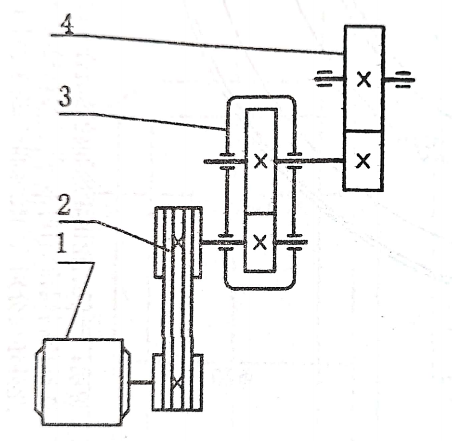
\includegraphics[width=0.5\textwidth]{figure/传动简图.png}
    \caption{传动简图草绘}
    \label{传动简图}
\end{figure}

caption是图片下面的注释,而label是可以用来索引的,比如我索引图片\ref{传动简图},使用ref命令;

可以用width=xx \textbackslash textwidth来设置图像大小

其他图像插入方法自行百度

\section{表格}

这块内容比较复杂。我自己掌握的比较好了,但总体来说还有欠缺;可以随时问我,比如:

% Please add the following required packages to your document preamble:
% \usepackage{graphicx}
\begin{table}[H]
\centering
\caption{总体设计大作业某个表格}
\resizebox{\textwidth}{!}{%
\begin{tabular}{|c|c|c|}
\hline
\textbf{部分名称} & \textbf{部分重量} & \textbf{部分重心位置(离机头)$/kg$} \\ \hline
\textbf{机身} & \textbf{$M_{FUS}=32555.4kg$} & \textbf{$x_{FUS}=\frac{66.18}{2}=33.08m$} \\ \hline
\textbf{机翼} & \textbf{$M_{w}=20572.37kg$} & \textbf{$x_{w}=30.1717m$} \\ \hline
\textbf{水平尾翼} & \textbf{$M_{H}=2042.42kg$} & \textbf{$x_{H}=64.328m$} \\ \hline
\textbf{垂直尾翼} & \textbf{$M_{V}=928.00kg$} & \textbf{$x_{V}=64.263m$} \\ \hline
\textbf{起落装置} & \textbf{$M_{lg}=11792.9kg$} & \textbf{$x_{lg}=x_G$} \\ \hline
\textbf{动力装置} & \textbf{$M_{pow}=22704.2kg$} & \textbf{$x_{pow}=23.8197$} \\ \hline
\textbf{系统和设备} & \textbf{$M_{system}=29723.9kg$} & \textbf{$x_{system}=x_G$} \\ \hline
\textbf{使用项目} & \textbf{$M_{op}=6975kg$} & \textbf{$x_{op}=x_G$} \\ \hline
\textbf{有效载荷} & \textbf{$M_{eff}=33860kg$} & \textbf{$x_{eff}=30.7892m$} \\ \hline
\textbf{燃油} & \textbf{$M_f=79110.7kg$} & \textbf{$x_{f}=x_w=39.1717m$} \\ \hline
\textbf{全集总重与质心位置} & \textbf{$M_G=240264.89kg$} & \textbf{$x_G=m$} \\ \hline
\end{tabular}%
}
\end{table}

同样的可以对表格设置caption和label,一般跟在centering后面;不赘述


可以直接把excel复制到网址https://www.tablesgenerator.com/上,生成latex表格代码  %%  书写的时候请直接删除/注释这一行

\chapter{设计任务书} %%  飞机设计要求
\chapter{飞机总体布局} %%  飞机总体布局
\chapter{载荷计算和设计计算} %%  发动机选择
\chapter{传动零件的设计计算} %%  主要参数确定
\chapter{轴的计算} %%  机身设计
\chapter{键连接的选择和计算} %%  机翼设计
\chapter{滚动轴承的选择和计算} %%  尾翼设计
\chapter{联轴器的选择} %%  发动机短舱设计
\chapter{润滑与密封的选择、润滑剂牌号和装油量} %%  起落架布置
\chapter{飞机三视图} %%  飞机三视图
\chapter{重量特性} %%  重量特性
\chapter{气动特性} %%  气动特性
\chapter{性能特性} %%  性能特性
\chapter{个人总结} %%  个人总结

\begin{thebibliography}{99}
\addcontentsline{toc}{chapter}{参考文献}  %%  将“参考文献加入目录中”
\bibitem{1}{余雄庆, 徐惠民, 昂海松. 飞机总体设计[M].}
\bibitem{2}{李为吉. 现代飞机总体综合设计[M]. 西安:西北工业大学出版社,2001.}
\bibitem{3}{黄维娜, 李中祥. 国外航空发动机简明手册[M]. 西安:西北工业大学出版社,2014.}
\bibitem{4}{林左鸣. 世界航空发动机手册[M]. 北京:航空工业出版社,2012.}
\bibitem{5}{尚义.航空燃气涡轮发动机[M]. 航空工业出版社:北京,1995}
\bibitem{6}{Denis Howe. 飞机载荷与结构布局[M]. 北京:航空工业出版社,2014. 38.}
\bibitem{7}{L.R.Jenkinson, P.Simpkin, D.Rhodes. 民用喷气飞机设计[M]. 北京:航空工业出版社,2014. 121.}
\bibitem{8}{潘立军, 余雄庆. 民用飞机概念设计中客舱布置的工具开发[J]. 机械设计与制造工程, 2014(10):27-31.}
\bibitem{9}{潘立军,余雄庆.客机概念设计中主要参数初估的计算工具[J].民用飞机设计与研究,2015,(1):27-31,61. DOI:10.3969/j.issn.1674-9804.2015.01.007.}
\end{thebibliography} %%  参考文献
\chapter*{附录}
\addcontentsline{toc}{chapter}{附录}  %%  overleaf中打开时请取消该句注释!!!
\appendix

\renewcommand{\thesection}{\Alph{section}}


\section{绘图程序代码}

\subsection{matlab绘制程序}

\lstinputlisting[language=matlab]{code/plot.m}  %%  附录

\end{document}
